\scanpage{435}

\unsure{lié} de façon beaucoup plus naturelle \unsure{à} la structure
$\overline{\mathrm m}$ du groupe $\mathcal{M}_{\rho,\sigma}$ et à ses hom.
$\xrightarrow{\Theta}G$ et $\chi=\det\circ\Theta$ dans $G_m$, savoir le
ss-groupe \unsure{entier} $SR_{\rho,\sigma}$, permettant d'écrire
$\overline{\mathrm m}$ $\mathcal{M}_{\rho,\sigma}^{+}$ comme un
\uline{produit direct}
\[
\tag{99}
\begin{array}{rccccc}
\mathcal{M}_{\rho,\sigma}^{+}&\simeq&SR_{\rho,\sigma}&\times&
 \unsure{\mathcal{G}|\mathcal{C}}_{\rho,\sigma}^{+}\\
&&\rotatebox{90}{$\simeq$}&&\rotatebox{90}{$\simeq$}\\
&&S'T_\rho\times SN'_\sigma&&SG
\end{array}
.
\]
induisant une décomposition analogue
\[
\tag{100}
\left\{
\begin{aligned}
\mathcal{M}_{\rho,\sigma}^{+\circ}
 &\simeq \underset{ST_\rho\times ST_\sigma}{\underbrace{
 SR_{\rho,\sigma}^{\deleted{\unsure{+}}\inserted{\circ}}}}
 \times
 \underset{SG}{\underbrace{\unsure{\mathcal{G}|\mathcal{C}}_{\rho,\sigma}^{+}}}\\
 &\simeq ST_\rho\times ST_\sigma\times SG,
\end{aligned}
\right.
\]
\margin{C'est (46), que j'avais oublié chemin faisant\ldots}
qui dit mieux !. D'autre part, le fait que
$R_{\rho,\sigma}\longrightarrow\mathcal{T}_{\rho,\sigma}$ soit une
\uline{isogénie} mod $\mu_2$ montre que l'on a, à cette isogénie près, une
``section'' \unsure{$\overline{\mathrm m}$}
\deleted{de $\unsure{\mathcal{T}_\rho}$}
\inserted{$\mathcal{M}_{\rho,\sigma}$ lui $\overline{\mathrm m}$}
en tant qu'extension de $\mathcal{T}_{\rho,\sigma}$ par
$\unsure{\mathcal{G}|\mathcal{C}}_{\rho,\sigma}^{+}\simeq SG$.
En fait, on a
\[
\tag{101}
\left\{
\begin{array}{l}
R_{\rho,\sigma}\cap SG=\mu_2\\[4pt]
\deleted{\text{\unsure{mais} }R_{\rho,\sigma}\text{ \unsure{ne commute plus},}}\\[-2pt]
\deleted{\text{\unsure{donc on a une suite exacte}}}\\[4pt]
R_{\rho,\sigma}\text{ commute à }SG
\end{array}
\right.
\]
\hfill (trivial par définition de $R_{\rho,\sigma}$ comme
$\operatorname{Ker}\widetilde{\Theta}$

donc on a une suite exacte

\mspage{434}

\begin{center}
{\small
434\\
\texttt{https://grothendieck.umontpellier.fr}\\
Université de Montpellier, UMR CNRS 5149, Case courrier 051, Place Eugène Bataillon\\
34095 Montpellier cedex 5 - France
}
\end{center}

\scanpage{436}
\mspage{520}

\noindent(102)
\diagram{\begin{tikzcd}[ampersand replacement=\&,column sep=large,row sep=small]
1\arrow[r]\&\mu_2\arrow[r]\&R_{\rho,\sigma}\times SG\arrow[r]\&
 \mathcal{M}_{\rho,\sigma}\arrow[r]\&1\\
\&\varepsilon\arrow[r,mapsto]\&
 \left(\varepsilon,
 \underset{\inserted{\substack{\Vert\\\varepsilon^{-1}}}}
 {\varepsilon^{\deleted{\unsure{+}}}}\right)
\end{tikzcd}}

et de même

\noindent(103)
\diagram{\begin{tikzcd}[ampersand replacement=\&,column sep=large]
1\arrow[r]\&\mu_2\arrow[r]\&R_{\rho,\sigma}^{\circ}\times SG\arrow[r]\&
\mathcal{M}_{\rho,\sigma}^{\circ}\arrow[r]\&1
\end{tikzcd}}

déjà envisagée (un peu timidement) dans (78).
C'est le moment décidément d'expliciter entièrement la description de
$R_{\rho,\sigma}$ en termes de $T_\rho,N'_\sigma\ldots$ --- on l'obtient,
dans le contexte de la p.~510, \deleted{comme} comme
\[
\tag{104}
\begin{aligned}
R_{\rho,\sigma}
={}&\left\{
 \left(
 \underset{\substack{\rotatebox{90}{$\in$}\\\Gamma T_0}}{\underline u},
 \underset{\substack{\rotatebox{90}{$\in$}\\\Gamma T_\rho}}{\underline a},
 \underset{\substack{\rotatebox{90}{$\in$}\\\unsure{\Gamma N'_\sigma|\Gamma^{*}N'_\sigma}}}{\underline b}
 \right)\cdot
 \underset{\substack{\rotatebox{90}{$\in$}\\SG}}{f}
 \ \middle|\ 
 \begin{gathered}
 \det\underline u=\det\underline b=\varepsilon'\det\underline a,
 \quad\varepsilon'{}^2=1\\
 \underline u f=\lambda\qquad(\varepsilon',\lambda\in\Gamma G_m)\\
 (\text{d'où }\lambda^2=\det\underline u)
 \end{gathered}\right\}\\[8pt]
\simeq{}&\left\{
 \left(\underset{T_0}{\underline u},
       \underset{T_\rho}{\underline a},
       \underset{N'_\sigma}{\underline b}\deleted{\unsure{)}},
       \underset{G_m}{\lambda}\right)
 \ \middle|\ \det\underline u=\det\underline b
 =\varepsilon'\det\underline a=\lambda^2\right\}\\[8pt]
\simeq{}&\left\{
 \left(\underset{T_\rho}{\underline a},
       \underset{N'_\sigma}{\underline b},
       \underset{G_m}{\lambda}\deleted{\unsure{)}},
       \inserted{\underset{\mu_2}{\varepsilon'}}\right)
 \ \middle|\
 \begin{gathered}
 \inserted{\det\underline b=\varepsilon'\det\underline a=\lambda^2}\\
 \deleted{\unsure{\det\underline b/\det\underline a\in\Gamma\mu_2}}
 \end{gathered}\right\}\\[8pt]
\simeq{}&\left\{
 \left(\underset{T_\rho}{\underline a},
       \underset{N'_\sigma}{\underline b},
       \underset{G_m}{\lambda}\right)
 \ \middle|\ \det\underline b=\lambda^2,\quad
 \det\underline a^2=\det\underline b^2\right\}\\[8pt]
\simeq{}&\left(\deleted{\unsure{\{}}(T_\rho,\delta_\rho^2)
 \times_{G_m}(N'_\sigma,\delta_\sigma^2)\right)_{(\delta_\sigma)}
 \times_{G_m}G_m{}_{(\delta^2)}
\end{aligned}
\]
ou plus simplement, \deleted{ce qui donne}
\inserted{en termes de $\mathcal{T}_{\rho,\sigma}$ :}
\[
\deleted{(105)\qquad
\begin{aligned}
 R_{\rho,\sigma}^{\circ}
 &\simeq\left\{
 \left(\underset{T_\rho}{\underline a},
       \underset{T_\sigma}{\underline b},
       \underset{G_m}{\lambda}\right)
 \ \middle|\ \det\underline a=\det\underline b=\lambda^2
 \right\}\\
 &\simeq\unsure{\mathcal{G}|\mathcal{C}}_{\rho,\sigma}^{\circ}
\end{aligned}}
\]

\noindent(105')
\diagram{\begin{tikzcd}[ampersand replacement=\&,column sep=large,row sep=large]
R_{\rho,\sigma}\arrow[r]\arrow[d,"{\kappa}"']\&
 \mathcal{T}_{\rho,\sigma}\arrow[d,"{\chi}"]\&\text{diagramme}\\
G_m\arrow[r,"{\delta^2}"']\&G_m\&\text{cartésien}\\[-1em]
\lambda\arrow[r,mapsto]\&\lambda^2
\end{tikzcd}},

\mspage{435}

\begin{center}
{\small
435\\
\texttt{https://grothendieck.umontpellier.fr}\\
Université de Montpellier, UMR CNRS 5149, Case courrier 051, Place Eugène Bataillon\\
34095 Montpellier cedex 5 - France
}
\end{center}

\scanpage{437}

s'insérant dans un diagramme de suites exactes

\noindent(106)
\diagram{\begin{tikzcd}[ampersand replacement=\&,column sep=large,row sep=large]
\&\&1\arrow[d]\&1\arrow[d]\&\\
\deleted{\unsure{1}}\arrow[r,draw=none,"{\deleted{\longrightarrow}}" description]\&
\deleted{\unsure{\mu_2}}\arrow[r,draw=none,"{\deleted{\longrightarrow}}" description]\&
SR_{\rho,\sigma}\arrow[r,"{\simeq}"]\arrow[d]\arrow[dr,phantom,"{*}" description]\&
\mathcal{T}_{\rho,\sigma}^{+}\arrow[d]
 \arrow[r,draw=none,"{\deleted{\longrightarrow}}" description]\&\deleted{1}\\
1\arrow[r]\&\mu_2\arrow[r]\arrow[d,equal]\&
R_{\rho,\sigma}\arrow[r,"{\mathrm{can.}}"]\arrow[d,"{\kappa}"]\&
\mathcal{T}_{\rho,\sigma}\arrow[r]\arrow[d,"{\chi}"]\&1\\
1\arrow[r]\&\mu_2\arrow[r]\&G_m\arrow[r,"{\lambda\mapsto\lambda^2}"]\arrow[d]\&
G_m\arrow[r]\arrow[d]\&1\\
\&\&1\&1\&
\end{tikzcd}}

qui n'est qu'une explicitation de la face supérieure
\inserted{$(*)$} des diagrammes cubiques (96) ---
\deleted{\unsure{donc}} \unsure{on} fera \unsure{attention} que celle-ci
\inserted{n'est \uline{pas} cartésienne} --- ni la face inférieure.
Ainsi, on construit
\deleted{$\unsure{\mathcal{T}_{\rho,\sigma}}$ et
$\unsure{\mathcal{T}_{\rho,\sigma}|R_{\rho,\sigma}}$}

\noindent(107) groupe $\mathcal{T}_{\rho,\sigma}$, et \inserted{les hom.}
\diagram{\begin{tikzcd}[ampersand replacement=\&,column sep=large]
\mathcal{T}_{\rho,\sigma}\arrow[r,"{\chi}"]\&G_m
\end{tikzcd}},
\diagram{\begin{tikzcd}[ampersand replacement=\&,column sep=large]
\mathcal{T}_{\rho,\sigma}\arrow[r,"{{(\varepsilon_3,\varepsilon_2)}}"]\&\mu_2\times\mu_2
\end{tikzcd}}

[et par là \unsure{(grâce à} (105')---(106)) $R_{\rho,\sigma}$,
$SR_{\rho,\sigma}\simeq\mathcal{T}_{\rho,\sigma}^{+}$, et aussi
(en \deleted{\unsure{simplifiant}}\inserted{remplaçant}
$\mathcal{T}_{\rho,\sigma}$ par
$\mathcal{T}_{\rho,\sigma}^{\circ}=\operatorname{Ker}
(\mathcal{T}_{\rho,\sigma}\longrightarrow\mu_2\times\mu_2)$)
$R_{\rho,\sigma}^{\circ}$,
$SR_{\rho,\sigma}^{\circ}\simeq\mathcal{T}_{\rho,\sigma}^{+\circ}$
\unsure{$\Rightarrow$}]
en termes des groupes

\noindent(108) $T_\rho,N'_\sigma$ et de
\diagram{\begin{tikzcd}[ampersand replacement=\&,column sep=large]
T_\rho\arrow[r,"{\delta_\rho}"]\&G_m
\end{tikzcd}},
\diagram{\begin{tikzcd}[ampersand replacement=\&,column sep=large,row sep=large]
N'_\sigma\arrow[r,"{\delta_\sigma}"]\&G_m\\
N'_\sigma\arrow[r,"{\varepsilon_\sigma}"]\&\mu_2
\end{tikzcd}},

\mspage{436}

\begin{center}
{\small
436\\
\texttt{https://grothendieck.umontpellier.fr}\\
Université de Montpellier, UMR CNRS 5149, Case courrier 051, Place Eugène Bataillon\\
34095 Montpellier cedex 5 - France
}
\end{center}

\scanpage{438}
\mspage{521}

comme sous-groupe

\noindent(109)
\diagram{\begin{tikzcd}[ampersand replacement=\&,column sep=small,row sep=large]
\mathcal{T}_{\rho,\sigma}\arrow[r,hook]\&
T_0\arrow[d,"{\delta_0}","{\simeq}"']\&{}\times T_\rho\times N'_\sigma\\
\&G_m\&
\end{tikzcd}}
\[
\begin{aligned}
&\phantom{\{}\,\Vert\\[-2pt]
&\left\{\left(\underset{T_0}{\underline u},
              \underset{T_\rho}{\underline a},
              \underset{N'_\sigma}{\underline b}\right)
 \ \middle|\ 
 \delta_0(\underline u)=\delta_\sigma(\underline b)
 =\varepsilon'\delta_\rho(\underline a),\quad\varepsilon'{}^2=1
 \right\}\\
&\hspace{3em}\simeq
 \left\{\left(\underset{T_\rho}{\underline a},
              \underset{N'_\sigma}{\underline b}\right)
 \ \middle|\
 \delta_\rho(\underline a)=\varepsilon'\delta_\sigma(\underline b),
 \quad\varepsilon'{}^2=1\right\}
\end{aligned}
\]
avec
\[
\tag{110}
\left\{
\begin{aligned}
\chi(\deleted{\underline u,}\underline a,\underline b)
 &=\unsure{\delta_\sigma|\delta_0}(\underline b)\\
\varepsilon_3(\deleted{\underline u,}\underline a,\underline b)
 &=\delta_\rho(\underline a)/\delta_\sigma(\underline b)\\
\varepsilon_2(\deleted{\underline u,}\underline a,\underline b)
 &=\varepsilon_\sigma(\underline b)
\end{aligned}
\right.
.
\]

À l'aide de ceci, on peut construire $\mathcal{M}_{\rho,\sigma}$
par (102), et bien entendu l'hom

\noindent(111) $\Theta:$\quad
\diagram{\begin{tikzcd}[ampersand replacement=\&,column sep=large]
\mathcal{M}_{\rho,\sigma}\arrow[r]\&G
\end{tikzcd}}

est déduit \unsure{par} passage au quotient des hom évidents

\noindent(112)
\diagram{\begin{tikzcd}[ampersand replacement=\&,column sep=large]
SG\arrow[r,hook]\&G
\end{tikzcd}},\qquad
\diagram{\begin{tikzcd}[ampersand replacement=\&,column sep=large,row sep=large]
R_{\rho,\sigma}\arrow[rr]\arrow[dr,"{\kappa}"']\&\&G\\
\&G_m\arrow[r,"{\simeq}"']\&
\uline{\operatorname{Centr}}(G)\arrow[u,hook]
\end{tikzcd}}

\deleted{On n'a pas eu à}
d'où on déduit les composés

\noindent(113)
\diagram{$\left\{\vcenter{\hbox{\begin{tikzcd}[ampersand replacement=\&,column sep=large,row sep=huge]
\mathcal{M}_{\rho,\sigma}\arrow[r,"{\Theta}"]
 \arrow[rr,bend right=25,"{\widetilde{\Theta}}"']\&
 G\arrow[r]\&PG\\
\mathcal{M}_{\rho,\sigma}\arrow[r,"{\Theta}"]
 \arrow[rr,bend right=25,"{\chi}"']\&
 G\arrow[r,"{\det}"]\&G_m
\end{tikzcd}}}\right.$}

On déduit aussi la suite exacte

\noindent(114)
\diagram{\begin{tikzcd}[ampersand replacement=\&,column sep=large,row sep=large]
1\arrow[r]\&SG\arrow[rr,"{\mathrm{can}}"']\arrow[dr,dashed,"{\mathrm{can}}"']\&\&
\mathcal{M}_{\rho,\sigma}\arrow[r]\&
\mathcal{T}_{\rho,\sigma}\arrow[r]
 \arrow[d,phantom,"{{\rotatebox{90}{$\simeq$}}}" description]\&1\\
\&\&R_{\rho,\sigma}\times SG\arrow[ur,dashed,"{\mathrm{can}}"]\&\&
R_{\rho,\sigma}/\mu_2\&
\end{tikzcd}}

\mspage{437}

\begin{center}
{\small
437\\
\texttt{https://grothendieck.umontpellier.fr}\\
Université de Montpellier, UMR CNRS 5149, Case courrier 051, Place Eugène Bataillon\\
34095 Montpellier cedex 5 - France
}
\end{center}

\scanpage{439}

de la description (102), d'où des composés

\noindent (115)
\diagram{\begin{tikzcd}[ampersand replacement=\&,column sep=large,row sep=small]
 \& \& T_\rho \\
\mathcal{M}_{\rho,\sigma}\arrow[r]
 \& \mathcal{T}_{\rho,\sigma}
   \arrow[ur,"{\mathrm{pr}_1}"]
   \arrow[dr,"{\mathrm{pr}_2}"]
   \arrow[ddr]
 \& \& \\
 \& \& N'_\sigma\arrow[r,"{\det}"] \& G_m \\
 \& \& \mu_2\times\mu_2
\end{tikzcd}}

Dans tout ceci, on n'a pas eu besoin de la donnée des sections $\rho,\sigma$
de $G$, ni de connaître quoi que ce soit de la façon dont $T_\rho,N'_\sigma$
\deleted{sont}\inserted{ont été} obtenus à partir de telles sections.
Mais des structures \unsure{supplémentaires} plus délicates des
$\mathcal{M}_{\rho,\sigma}$ --- telle la donnée des ss-groupes
\unsure{entiers} $\mathcal{M}_{\rho,\sigma}\unsure{(w)|(\omega)}$ ---
en dépendent, et permettront peut-être de les retrouver.

\uline{\unsure{Remq.|Rem.}} Le cube (96) est le "composé" de deux diagrammes
cubiques, que je vais expliciter, dont le premier complète (95) --- qui peut
être considéré comme un diagramme partiel de celui-ci :

\mspage{438}

\begin{center}
{\small
438\\
\texttt{https://grothendieck.umontpellier.fr}\\
Université de Montpellier, UMR CNRS 5149, Case courrier 051, Place Eugène Bataillon\\
34095 Montpellier cedex 5 - France
}
\end{center}

\scanpage{440}
\mspage{522}

\noindent (116)
\diagram{\begin{tikzcd}[ampersand replacement=\&,column sep=small,row sep=small]
 \& \& G_m\arrow[ddrr,dashed,"{\lambda\mapsto\lambda^2}"] \& \& \\
 \& R_{\rho,\sigma}
       \arrow[ur,dashed,"{\kappa}"]
       \arrow[drr,hook,"{PG}"]
 \& \& \& \\
 SR_{\rho,\sigma}
       \arrow[ur,hook,"{G_m}"]
       \arrow[rrr,dashed,"{G}"]
       \arrow[ddrr,hook,"{SG}"']
 \& \& \& \mathcal{M}_{\rho,\sigma}\arrow[r,dashed,"{\chi}"] \& G_m \\
 \& \& \& \& \\
 \& \& \mathcal{M}_{\rho,\sigma}^{+}
       \arrow[uur,hook,"{G_m}"]
 \& G_m\arrow[ddr,dashed,"{\lambda\mapsto\lambda^2}"] \& \\
 \& R_{\rho,\sigma}^{\circ}
       \arrow[uuuu,hook,"{\mu_2\times\mu_2}"]
       \arrow[urr,dashed,"{\kappa^{\circ}}"']
       \arrow[drr,hook,"{PG}"]
 \& \& \& \\
 SR_{\rho,\sigma}^{\circ}
       \arrow[uuuu,hook,"{\mu_2\times\mu_2}"']
       \arrow[ur,hook,"{G_m}"]
       \arrow[rrr,dashed,"{G}"]
       \arrow[ddrr,hook,"{SG}"']
 \& \& \& \mathcal{M}_{\rho,\sigma}^{\circ}
       \arrow[uuuu,hook,"{\mu_2\times\mu_2}"]
       \arrow[r,dashed,"{\chi^{\circ}}"]
 \& G_m \\
 \& \& \& \& \\
 \& \& \mathcal{M}_{\rho,\sigma}^{+\circ}
       \arrow[uuuu,hook,
        "{\begin{gathered}\inserted{\mu_2\times\mu_2}\\
        \deleted{\unsure{\mu_2\times\mu_2}}\end{gathered}}"']
       \arrow[uur,hook,"{G_m}"]
 \& \& \\
 \& \& \rotatebox{90}{$\simeq$} \& \&
\end{tikzcd}}

Comme dans (95)(96), la face inférieure est déduite de la supérieure en
\unsure{passant} aux composantes neutres, les quatre groupes quotients sont
isom entre eux par les flèches can, ils sont isomorphes à
$\mu_2\times\mu_2$ --- \unsure{idem} dans le cube \inserted{accolé}
ci-dessous (117). Les faces latérales du cube sont cart. et.
cocartésiennes, mais pas les faces sup. ni la face inf.

\mspage{439}

\begin{center}
{\small
439\\
\texttt{https://grothendieck.umontpellier.fr}\\
Université de Montpellier, UMR CNRS 5149, Case courrier 051, Place Eugène Bataillon\\
34095 Montpellier cedex 5 - France
}
\end{center}

\scanpage{441}
\mspage{523}

\[
\tag{117}
\diagram{\begin{tikzcd}[ampersand replacement=\&,column sep=1.5em,row sep=2.5em]
 \& \& R_{\rho,\sigma}\arrow[drr,hook,"{{PG}}"] \& \& \& \\
 SR_{\rho,\sigma}\arrow[urr,hook,"{{G_m}}"]\arrow[rrrr,dashed,"{{G}}"]\arrow[dr,hook,"{{SG}}"'] \& \& \& \& \mathcal M_{\rho,\sigma}\arrow[dr,hook] \& \\
 \& \begin{gathered}\mathcal M_{\rho,\sigma}^{+}\\[-.3em]\inserted{\unsure{\simeq SR_{\rho,\sigma}\times SG}}\end{gathered}\arrow[urrr,hook,"{{G_m}}"]\arrow[drr,shift left=.6ex] \& \& \& \& \mathcal T_{\rho,\sigma} \\
 \& \& R_{\rho,\sigma}^{\circ}\arrow[uuu,hook,"{{\mu_2\times\mu_2}}",description,pos=.6]\arrow[drr,hook,"{{\unsure{SG|PG}}}"] \& \mathcal T_{\rho,\sigma}^{+}\arrow[urr,hook,"{{G_m}}"]\arrow[ull,shift left=.6ex] \& \& \\
 \begin{gathered}SR_{\rho,\sigma}^{\circ}\\[-.5em]\rotatebox{90}{$\simeq$}\\[-.5em]ST_\rho\times ST_\sigma\end{gathered}\arrow[uuu,hook,"{{\mu_2\times\mu_2}}"']\arrow[urr,hook,"{{G_m}}"]\arrow[rrrr,dashed,"{{G}}"]\arrow[dr,hook,"{{SG}}"'] \& \& \& \& \mathcal M_{\rho,\sigma}^{\circ}\arrow[uuu,hook,"{{\mu_2\times\mu_2}}",description]\arrow[dr] \& \\
 \& \mathcal M_{\rho,\sigma}^{+\circ}\arrow[uuu,hook,"{{\mu_2\times\mu_2}}"']\arrow[urrr,hook,"{{G_m}}"] \& \& \& \& \mathcal T_{\rho,\sigma}^{\circ}\arrow[uuu,hook,"{{\mu_2\times\mu_2}}"] \\
 \& \& \& \begin{gathered}\mathcal T_{\rho,\sigma}^{+\circ}\\[-.5em]\rotatebox{90}{$\simeq$}\\[-.5em]ST_\rho\times ST_\sigma\end{gathered}\arrow[uuu,hook,"{{\mu_2\times\mu_2}}"]\arrow[ull]\arrow[urr,hook,"{{G_m}}"'] \& \&
\end{tikzcd}}
\]

La face \unsure{oblique} antérieure gauche du cube est de nature particulièrement simple, puisque les termes médians $\mathcal M_{\rho,\sigma}^{+}$, $\mathcal M_{\rho,\sigma}^{+\circ}$ s'identifient \unsure{simplement} aux produits directs des termes extrêmes
\[
\begin{gathered}
SR_{\rho,\sigma}\xrightarrow{\sim}\mathcal T_{\rho,\sigma}^{+}
\quad\text{et}\quad
SR_{\rho,\sigma}^{\circ}\xrightarrow{\sim}\mathcal T_{\rho,\sigma}^{+\circ}\\
\hphantom{SR_{\rho,\sigma}\xrightarrow{\sim}}\simeq S'T_\rho\times SN'_\sigma
\qquad\qquad\simeq ST_\rho\times ST_\sigma
\end{gathered}
\]
avec le groupe $SG$. C'est presque le cas aussi pour la face parallèle (face postérieure droite), \inserted{au groupe $\mu_2$ près -- cela devient vrai \unsure{à}} à condition de remplacer les \deleted{groupes $\mathcal M_{\rho,\sigma}$} termes médians $\mathcal M_{\rho,\sigma}$, $\mathcal M_{\rho,\sigma}^{\circ}$ par les $\mu_2$-revêtements
\[
\tag{118}
\mathcal M_{\rho,\sigma}^{\sim}\simeq\unsure{R}_{\rho,\sigma}\times SG,
\qquad \mathcal M_{\rho,\sigma}^{\circ\sim}\simeq R_{\rho,\sigma}^{\circ}\times SG
\]
(cf. (102), (103)), ce qui \unsure{aura} aussi la vertu

\mspage{440}

\begin{center}
{\small
440\\
\texttt{https://grothendieck.umontpellier.fr}\\
Université de Montpellier, UMR CNRS 5149, Case courrier 051, Place Eugène Bataillon\\
34095 Montpellier cedex 5 - France
}
\end{center}

\scanpage{442}

\unsure{délectable} de rendre les quatre carrés des faces sup. et inférieures des deux cubes accolés cartésiens et cocartésiens, ce qu'ils n'étaient pas avant, \unsure{regrettablement}.

Pour terminer ces gammes sur les \unsure{radicaux} je vais introduire un hom canonique
\[
\tag{118}
\diagram{\begin{tikzcd}[ampersand replacement=\&]
G_m\arrow[r,hook,"{{i_R}}"] \& R_{\rho,\sigma}^{\circ}
\end{tikzcd}}
\]
via un hom canonique
\[
\tag{119}
\diagram{\begin{tikzcd}[ampersand replacement=\&,row sep=1em]
G_m\arrow[r,hook,"{{i_{\mathcal T}}}"] \& \mathcal T_{\rho,\sigma}^{\circ}\simeq T_\rho\times_{G_m}T_\sigma \\
\lambda\arrow[r,mapsto] \& (\lambda,\lambda)
\end{tikzcd}}
\]
dont la composée
\[
\diagram{\begin{tikzcd}[ampersand replacement=\&]
\chi:\mathcal T_{\rho,\sigma}^{\circ}\arrow[r] \& G_m
\end{tikzcd}}
\]
est donnée en effet par $\lambda\mapsto\lambda^2$ \inserted{\unsure{(104)|(109)}}, de sorte que grâce à la description (105) de $R_{\rho,\sigma}$ \inserted{en termes de $\mathcal T_{\rho,\sigma}$} comme produit fibré (\unsure{paraphrasée} en une expression de $R_{\rho,\sigma}^{\circ}$ en termes de $\mathcal T_{\rho,\sigma}^{\circ}$) on a un unique hom (118), rendant commutatif le diagramme

\mspage{441}

\begin{center}
{\small
441\\
\texttt{https://grothendieck.umontpellier.fr}\\
Université de Montpellier, UMR CNRS 5149, Case courrier 051, Place Eugène Bataillon\\
34095 Montpellier cedex 5 - France
}
\end{center}

\scanpage{443}
\mspage{524}

\[
\tag{120}
\diagram{\begin{tikzcd}[ampersand replacement=\&,column sep=3em,row sep=2em]
G_m\arrow[r,"{{i_{\mathcal T}}}"]\arrow[dr,"{{i_R}}"'] \& \mathcal T_{\rho,\sigma}^{\circ} \\
\& R_{\rho,\sigma}^{\circ}\arrow[u,"{{\mathrm{can}}}"']
\end{tikzcd}}
\]
ou, plus \unsure{pleinement|joliment}, le diagramme de suites exactes
\[
\tag{121}
\diagram{\begin{tikzcd}[ampersand replacement=\&,column sep=1.8em,row sep=2em]
1\arrow[r] \& \mu_2\arrow[r] \& G_m\arrow[r,"{{\lambda\mapsto\lambda^2}}"]\arrow[d,no head] \& G_m\arrow[r,no head] \& 1 \\
\& \& {} \& \&
\end{tikzcd}}.
\]

Par construction, on trouve aussitôt
\[
\tag{122}
\diagram{\begin{tikzcd}[ampersand replacement=\&,column sep=3em]
G_m\arrow[r,"{{i_R}}"]\arrow[rr,bend right=28,"{{\mathrm{id}}}"'] \& R_{\rho,\sigma}^{\circ}\arrow[r,"{{\kappa}}"] \& G_m
\end{tikzcd}}
\]
d'où des décompositions en produit direct
\[
\tag{123}
\left\{\begin{aligned}
R_{\rho,\sigma}&\simeq SR_{\rho,\sigma}\times G_m\simeq S'T_\rho\times SN'_\sigma\times G_m\\
R_{\rho,\sigma}^{\circ}&\simeq SR_{\rho,\sigma}^{\circ}\times G_m\\
&\simeq ST_\rho\times ST_\sigma\times G_m
\end{aligned}\right.,
\]
qui précise considérablement (96) dont j'étais pourtant si content !

En termes de cette décomposition, on va expliciter l'\deleted{\unsure{h}}hom
\[
\diagram{\begin{tikzcd}[ampersand replacement=\&,column sep=1.7em]
\mu_2\arrow[r,hook] \& R_{\rho,\sigma}^{\circ}\subset R_{\rho,\sigma}
\end{tikzcd}}
\quad
\left(\text{\unsure{et }}
\diagram{\begin{tikzcd}[ampersand replacement=\&,column sep=1.4em]
R_{\rho,\sigma}\arrow[r,no head] \& \mathcal T_{\rho,\sigma}
\end{tikzcd}},\ 
\diagram{\begin{tikzcd}[ampersand replacement=\&,column sep=1.4em]
R_{\rho,\sigma}^{\circ}\arrow[r] \& \mathcal T_{\rho,\sigma}^{\circ}
\end{tikzcd}}\right)
\]
qui intervient dans (102), (103), $\mu_2=R_{\rho,\sigma}\cap SG=R_{\rho,\sigma}^{\circ}\cap SG$,

\deleted{\unsure{On trouve} dans l'explicitation (104), que $\mu_2$ correspond aux $\varepsilon\in\Gamma\mu_2$, \unsure{que} \illegible{3}}

\mspage{442}

\begin{center}
{\small
442\\
\texttt{https://grothendieck.umontpellier.fr}\\
Université de Montpellier, UMR CNRS 5149, Case courrier 051, Place Eugène Bataillon\\
34095 Montpellier cedex 5 - France
}
\end{center}

\scanpage{444}

Pour l'hom
\[
\diagram{\begin{tikzcd}[ampersand replacement=\&,column sep=2em]
R_{\rho,\sigma}\arrow[r] \&
\begin{gathered}
\inserted{\{(\underline a,\underline b)\mid(\det\underline a/\det\underline b)^2=1\}}\\[-.5em]
\rotatebox{90}{$=$}\\[-.5em]
T_{\rho,\sigma}
\end{gathered}\arrow[r,hook] \& T_\rho\times N'_\sigma
\end{tikzcd}}
\]
il suffit de \deleted{définir} \inserted{expliciter} les composés
\[
\tag{124}
\left\{\begin{gathered}
\diagram{\begin{tikzcd}[ampersand replacement=\&,column sep=2.2em,row sep=1em]
\& \& T_\rho \\
R_{\rho,\sigma}\arrow[r]\arrow[d,phantom,"{{\rotatebox{90}{$\simeq$}}}" description] \& \unsure{T_{\sigma\sigma}|T_{\rho,\sigma}}\arrow[ur]\arrow[dr] \& \\
S'T_\rho\times SN'_\sigma\times G_m \& \& N'_\sigma
\end{tikzcd}}\\[1em]
\diagram{\begin{tikzcd}[ampersand replacement=\&]
(\underline a,\underline b,\lambda)\arrow[r] \& (\lambda\underline a,\lambda\underline b)
\end{tikzcd}}
\end{gathered}\right.
\]
\margin{on a aussi bien
\[
\underbrace{\det(\lambda\underline a)^2}_{\substack{\lambda^2\\\text{car }(\det\underline a)^2=1}}
=
\underbrace{\det(\lambda\underline b)^2}_{\substack{\lambda^2\ \text{car}\\\det\underline b=1}}
\]}

Le noyau de cet hom est donc formé des $(\unsure{\lambda}^{-1},\lambda^{-1},\lambda)$, où $\lambda\in\Gamma G_m$ tel que $\lambda^{-1}\in\Gamma S'T_\rho$, $\lambda^{-1}\in\Gamma SN'_\sigma$, \deleted{\unsure{c.à.d.|et}} i.e. $(\lambda^2)^2=1$ et $\lambda^2=1$, soit $\lambda\in\Gamma\mu_2$. Donc
\[
\tag{125}
\left\{\begin{gathered}
\diagram{\begin{tikzcd}[ampersand replacement=\&,column sep=2em]
\begin{gathered}\mu_2\\[-.5em]\rotatebox{90}{$=$}\\[-.5em]R_{\rho,\sigma}\cap SG\end{gathered}\arrow[r,"{{\mathrm{can}}}"] \&
\underbrace{R_{\rho,\sigma}^{\circ}}_{ST_\rho\times ST_\sigma\times G_m}\subset
\underbrace{R_{\rho,\sigma}}_{S'T_\rho\times SN'_\sigma\times G_m}
\end{tikzcd}}\\[1em]
\diagram{\begin{tikzcd}[ampersand replacement=\&]
\lambda\arrow[r,mapsto] \& (\lambda,\lambda,\lambda)
\end{tikzcd}}
\end{gathered}\right.
\]

On trouve donc l'explicitation particulièrement simple
\[
\tag{126}
\diagram{\begin{tikzcd}[ampersand replacement=\&,column sep=0em,row sep=.8em]
\mathcal T_{\rho,\sigma}\simeq(S'T_\rho\times SN'_\sigma\times G_m)/ \& \mu_2 \\
\& \begin{gathered}\mu_2\ \text{envoyé ``diagonalement'' dans le}\\\text{produit triple}\end{gathered}\arrow[u]
\end{tikzcd}}
\]

On notera qu'on a des hom canoniques
\[
\diagram{\begin{tikzcd}[ampersand replacement=\&,column sep=1.2em]
\mu_2\arrow[r,no head] \& ST_\rho\subset S'T_\rho
\end{tikzcd}},\quad
\diagram{\begin{tikzcd}[ampersand replacement=\&,column sep=1.2em]
\mu_2\arrow[r] \& ST_\sigma\subset SN'_\sigma
\end{tikzcd}},\quad
\diagram{\begin{tikzcd}[ampersand replacement=\&,column sep=1.2em]
\mu_2\arrow[r,no head] \& G_m
\end{tikzcd}}
\]
(qui sont utilisés dans (125)) d'où
\[
\tag{127}
\left\{\begin{gathered}
\diagram{\begin{tikzcd}[ampersand replacement=\&,column sep=1.5em]
\mu_2\times\mu_2\times\mu_2\arrow[r] \&
\underbrace{ST_\rho\times ST_\sigma\times G_m}_{R_{\rho,\sigma}^{\circ}}\subset
\underbrace{S'T_\rho\times SN'_\sigma\times G_m}_{R_{\rho,\sigma}}
\end{tikzcd}}\\
\diagram{\begin{tikzcd}[ampersand replacement=\&]
(\lambda',\lambda'',\lambda)\arrow[r,mapsto] \& (\lambda',\lambda'',\lambda)
\end{tikzcd}}
\end{gathered}\right.
\]
qui n'est autre que (48))

\mspage{443}

\begin{center}
{\small
443\\
\texttt{https://grothendieck.umontpellier.fr}\\
Université de Montpellier, UMR CNRS 5149, Case courrier 051, Place Eugène Bataillon\\
34095 Montpellier cedex 5 - France
}
\end{center}

\scanpage{445}
\mspage{525}

\uline{Le Centre de} $\mathcal M_{\rho,\sigma}$. Il s'envoie par $\widetilde\Theta$ dans le centre de $PG$ qui est trivial, donc
\[
\uline{\mathrm{Cent}}(\mathcal M_{\rho,\sigma})\subset\operatorname{Ker}\widetilde\Theta
=R_{\rho,\sigma}\simeq S'T_\rho\times SN'_\sigma\times G_m
\]
\unsure{d'où} évidemment. Comme $R_{\rho,\sigma}$ commute à $SG$, et que $R_{\rho,\sigma}\,\unsure{\cdot}\,SG=\mathcal M_{\rho,\sigma}$, on en conclut
\[
\tag{128}
\uline{\mathrm{Cent}}(\mathcal M_{\rho,\sigma})
=\uline{\mathrm{Cent}}(R_{\rho,\sigma})
=S'T_\rho\times\underset{?}{\uline{\mathrm{Cent}}}(SN'_\sigma)\times G_m
\]
déterminons donc $\mathrm{Cent}(SN'_\sigma)$. Notons que
\[
\left\{\begin{array}{l}
\mu_2\simeq N'_\sigma/T_\sigma\quad\text{opère fidèlement sur }T_\sigma\\
\text{et }T_\sigma=G_m.ST_\sigma
\end{array}\right.
\qquad
\begin{array}{|l}
\text{donc }\underset{\substack{\rotatebox{90}{$\simeq$}\\SN'_\sigma/\unsure{T_\sigma}}}{\mu_2}\text{ opère fidèlement}\\
\text{sur }ST_\sigma
\end{array}
\]
d'où
\[
\tag{129}
\uline{\mathrm{Cent}}(SN'_\sigma)\subset ST_\sigma
\quad\text{d'où}\quad
\uline{\mathrm{Cent}}(SN'_\sigma)\simeq(ST_\sigma)^{\mu_2}.
\]

Or on constate que
\inserted{\[
\tag{130}
T_\sigma^{\mu_2}\simeq G_m
\]}
\deleted{\unsure{la section} $-1$ de $\mu_2$ opère sur $ST_\sigma$ par $x\longrightarrow x^{-1}$, ce qui montre que
\[
\uline{\mathrm{Cent}}(SN'_\sigma)\subset {}_2(ST_\sigma)
=\left\{\unsure{c}\sigma+d\ \middle|\ \begin{array}{l}
-\nu c^2+d^2=1\\
\nu c^2+d^2+2\sigma cd=0
\end{array}\right\}
\]
On a pour une section de ${}_2ST_\sigma$, \deleted{\unsure{que}}
\[
\begin{array}{ll}
g=c\sigma+d & \det g=-\nu c^2+d^2=1\\
&g^2=\nu c^2+d^2+2cd\sigma=1
\end{array}
\]
\[
\text{i.e.}\quad
\left\{\begin{array}{ll}
-\nu c^2+d^2=1 & \nu c^2+d^2=1\\
2cd=0 &
\end{array}\right.
\]
\deleted{d'où} i.e.
\[
\left\{\begin{array}{ll}
2\nu c^2=0 & \text{donc }2c^2=0\quad(\text{car }\nu\text{ inv}).\\
2cd=0 &\\
-\nu c^2+d^2=1 &
\end{array}\right.
\]
si $2$ inv. cela revient à
\[
\left\{\begin{array}{lll}
&c^2=0&\\
\deleted{\unsure{c^2=0}}&d^2=1&(\text{donc }d\text{ inv.})\\
\deleted{\unsure{d^2=1}}&\unsure{c}d=0&\text{donc }c=0
\end{array}\right.
\]
\unsure{donc}
\[
\boxed{c=0,\ d^2=1}\quad\text{i.e. }g\in\mu_2
\]
\unsure{pour|donc si} $2$ inv.}
\inserted{d'où}
\[
\tag{\unsure{131|129}}
\uline{\mathrm{Cent}}(SN'_\sigma)
=\unsure{ST_\sigma}^{\mu_2}
=ST_\sigma\cap G_m
\inserted{=\mu_2}\quad
\deleted{\text{si }2\text{ inv. sur }S.}
\]

\deleted{Dans le cas général on aura seulement
\[
\tag{130}
\mu_2\subset\uline{\mathrm{Cent}}(SN'_\sigma)
\]
et cette inclusion induit un iso sur les groupes de sections dans le cas où $2$ est \unsure{semi-régulier} de}

\mspage{444}

\begin{center}
{\small
444\\
\texttt{https://grothendieck.umontpellier.fr}\\
Université de Montpellier, UMR CNRS 5149, Case courrier 051, Place Eugène Bataillon\\
34095 Montpellier cedex 5 - France
}
\end{center}

\scanpage{446}

\deleted{$\uline{\mathcal O}_S$. Désignons par \deleted{$\unsure{\mu'_2}$}
\[
\tag{131}
\begin{gathered}
\mu'_2\subset ST_\sigma\\[-.5em]
\rotatebox{90}{$=$}\\[-.5em]
\deleted{\unsure{\uline{\mathrm{Cent}}}}(ST_\sigma)^{\mu_2}
\end{gathered}
\]
\unsure{ce|un} sous-groupe de}

d'où \unsure{finalt|finalement}, \unsure{savoir|soit}:
\[
\tag{128}
\underset{\unsure{=}}{\uline{\mathrm{Cent}}(\mathcal M_{\rho,\sigma})}
\simeq S'T_\rho\times\mu_2\times G_m
\subset R_{\rho,\sigma}\simeq S'T_\rho\times SN'_\sigma\times G_m
\]
d'où
\[
\tag{129}
\uline{\mathrm{Cent}}(\mathcal M_{\rho,\sigma})\cap\mathcal M_{\rho,\sigma}^{\circ}
=ST_\rho\times\mu_2\times G_m
\subset R_{\rho,\sigma}^{\circ}\simeq ST_\rho\times ST_\sigma\times G_m
\]

Revenons aux sections entières dans le cas modulaire absolu
\[
\tag{130}
R_{\rho,\sigma}(\mathbb Z)\simeq
\underbrace{S'T_\rho(\mathbb Z)}_{\unsure{T_\rho}(\mathbb Z)\simeq\mathbb Z/6\mathbb Z}
\times
\underbrace{SN'_\sigma(\mathbb Z)}_{T_\sigma(\mathbb Z)=\mathbb Z/4\mathbb Z}
\times
\underbrace{G_m(\mathbb Z)}_{\mu_2(\mathbb Z)\simeq\pm1}
\]
\[
\tag{131}
\begin{aligned}
\uline{\mathrm{Cent}}(\mathcal M_{\rho,\sigma})\unsure{[\mathbb Z]|(\mathbb Z)}
&\simeq S'(T_\rho\unsure{[\mathbb Z]|(\mathbb Z)})\times\mu_2(\mathbb Z)\times G_m(\mathbb Z)\\
&\simeq\mathbb Z/6\mathbb Z\times\{\pm1\}\times\{\pm1\}
\end{aligned}
\]
et pour mémoire (cf (75), p. 514)
\[
\tag{132}
\begin{aligned}
\underbrace{\uline{\mathrm{Cent}}(\mathcal M_{\rho,\sigma}^{\circ})}_{\substack{R_{\rho,\sigma}^{\circ}\\\simeq ST_\rho\times ST_\sigma\times G_m}}(\mathbb Z)
&\simeq ST_\rho(\mathbb Z)\times ST_\sigma(\mathbb Z)\times G_m(\mathbb Z)\\
&\simeq\mathbb Z/6\mathbb Z\times\mathbb Z/4\mathbb Z\times\{\pm1\}.
\end{aligned}
\]

En résumé, on a le diagramme d'inclusions \inserted{strictes} de schémas en groupes
\[
\tag{133}
\diagram{\begin{tikzcd}[ampersand replacement=\&,column sep=1.5em,row sep=5em]
\text{dim }3 \&
\begin{gathered}
\uline{\mathrm{Cent}}(\mathcal M_{\rho,\sigma}^{\circ})=R_{\rho,\sigma}^{\circ}\\
\simeq ST_\rho\times ST_\sigma\times G_m
\end{gathered}
\arrow[rr,hook,"{{{\substack{\text{(quotient}\\\mu_2\times\mu_2\text{)}}}}}"']
\& \&
\begin{gathered}
R_{\rho,\sigma}\\
\simeq S'T_\rho\times SN'_\sigma\times G_m
\end{gathered}
\&\text{dim }3\\
\text{dim }2\&
\begin{gathered}
\uline{\mathrm{Cent}}(\mathcal M_{\rho,\sigma})\cap\mathcal M_{\rho,\sigma}^{\circ}\\
=ST_\rho\times\mu_2\times G_m
\end{gathered}
\arrow[u,hook]\arrow[rr,hook,"{{{\substack{\text{(quotient}\\\mu_2\text{)}}}}}"']
\&\&
\begin{gathered}
\uline{\mathrm{Cent}}(\mathcal M_{\rho,\sigma})\\
\simeq S'T_\rho\times\deleted{\unsure{SN'_\sigma}}\inserted{\unsure{\mu_2}}\times G_m)
\end{gathered}
\arrow[u,hook]
\&\text{dim }2
\end{tikzcd}}
\]

\mspage{445}

\begin{center}
{\small
445\\
\texttt{https://grothendieck.umontpellier.fr}\\
Université de Montpellier, UMR CNRS 5149, Case courrier 051, Place Eugène Bataillon\\
34095 Montpellier cedex 5 - France
}
\end{center}

\scanpage{447}
\mspage{526}

valable dans le cas général -- et qui, dans le cas modulaire absolu, induit \unsure{sur} les points entiers des isomorphismes pour les deux flèches horizontales, \unsure{correspondant} resp. aux deux groupes
\[
\underset{\unsure{\text{et}}}{(134)}\quad
\left\{
\begin{aligned}
\uline{\mathrm{Cent}}(\mathcal{M}_{\rho,\sigma}^{\circ})(\mathbb{Z})
 &\simeq \mathbb{Z}/6\mathbb{Z}\times\mathbb{Z}/4\mathbb{Z}\times\{\pm1\}\qquad\text{et}\\
\uline{\mathrm{Cent}}(\mathcal{M}_{\rho,\sigma})(\mathbb{Z})
 &\simeq \mathbb{Z}/6\mathbb{Z}\times\{\pm1\}\times\{\pm1\}
\end{aligned}\right.
\]
qui en est un sous-groupe d'indice 2.

Enfin, pour mémoire \unsure{signalons} à nouveau le groupe
\[
(135)\qquad \deleted{\unsure{\mu_2\times}}\qquad
\Sigma=\{\pm1\}\times\{\pm1\}\times\{\pm1\}
\]
contenu dans $\uline{\mathrm{Cent}}(\mathcal{M}_{\rho,\sigma})(\mathbb{Z})$ (d'ordre 8, d'indice 3), qui joue un rôle particulier dans l'application arithmétique, puisqu'on aura un homomorphisme canonique
\[
(136)\qquad
\boxed{\diagram{\begin{tikzcd}[ampersand replacement=\&,column sep=large]
\mathcal{M}_{0,3}^{\sim}\arrow[r] \& \mathcal{M}_{\rho,\sigma}(\widehat{\mathbb{Z}})/\Sigma
\end{tikzcd}}}\,.
\]

\mspage{446}

\begin{center}
{\small
446\\
\texttt{https://grothendieck.umontpellier.fr}\\
Université de Montpellier, UMR CNRS 5149, Case courrier 051, Place Eugène Bataillon\\
34095 Montpellier cedex 5 - France
}
\end{center}

\scanpage{448}

\margin{\uline{\unsure{Où on définit}}\quad\uline{$\mathcal{M}_{\rho,\sigma}$}}

\textcircled{$7^\circ$}\quad Faisons une \unsure{liste|petite} \unsure{récapitulation|récapitulative} des principaux homomorphismes de groupes envisagés au cours de la section $6^\circ$, impliquant le groupe $\mathcal{M}_{\rho,\sigma}$
\[
(134)\qquad
\diagram{\begin{tikzcd}[ampersand replacement=\&,row sep=small,column sep=large]
 \& SG\arrow[dddr,"{j_G}"] \& \& G\arrow[r]\arrow[dr,"{\delta_G=\det_G}"] \& PG\\
 \& \& \& \& G_m\\
 \& S'T_\rho\arrow[dr,"{j_\rho}"] \& \& T_\rho\arrow[r,"{\delta_\rho=\det_{T_\rho}}"] \& G_m\\
\mu_2\arrow[uuur]\arrow[ur]\arrow[dr]\arrow[dddr]
 \& \& \mathcal{M}_{\rho,\sigma}\arrow[uuur,"{\Theta=\Theta_G}"]\arrow[ur,"{\Theta_\rho}"]\arrow[dr,"{\Theta_\sigma}"]\arrow[dddr,"{\varepsilon_3}"'] \& \& \\
 \& SN'_\sigma\arrow[ur,"{j_\sigma}"'] \& \& N'_\sigma\arrow[r,"{\delta'_\sigma=\det_{T_\sigma}}"]\arrow[dr,"{\varepsilon_\sigma}"] \& G_m\\
 \& \& \& \& \mu_2\\
 \& G_m\arrow[uuur,hook,"{j_\mu}"'] \& \& \mu_2 \&
\end{tikzcd}}
\]

Notons que ce diagramme se reconstruit (avec les propriétés essentielles que nous allons \unsure{passer} en \unsure{revue}) à partir des données
\[
(135)\quad
\left\{\begin{gathered}
\diagram{\begin{tikzcd}[ampersand replacement=\&,column sep=large]
G_m\arrow[r,"{i_\rho}"] \& T_\rho\arrow[r,"{\delta_\rho}"] \& G_m \& (\delta_\rho i_\rho(\lambda)=\lambda^2)
\end{tikzcd}}\\[1em]
\diagram{\begin{tikzcd}[ampersand replacement=\&,column sep=large]
G_m\arrow[r,"{i_\sigma}"] \& N'_\sigma\arrow[r,"{\delta_\sigma}"] \& G_m \& (\delta_\sigma i_\sigma(\lambda)=\lambda^2)
\end{tikzcd}}\\[1em]
\diagram{\begin{tikzcd}[ampersand replacement=\&,column sep=large]
 \& N'_\sigma\arrow[r,"{\varepsilon_\sigma}"] \& \mu_2 \& \varepsilon_\sigma i_\sigma(\lambda)=1
\end{tikzcd}}\\[1em]
\diagram{\deleted{\begin{tikzcd}[ampersand replacement=\&,column sep=large]
1\arrow[r] \& G_m\arrow[r]\arrow[dr,phantom,"{\text{cart}}" description] \& G\arrow[r] \& PG\arrow[r] \& 1\\
1\arrow[r] \& \mu_2\arrow[u,hook]\arrow[r] \& SG\arrow[u,hook]\arrow[r] \& PG\arrow[u,equal]\arrow[r] \& 1
\end{tikzcd}}}
\end{gathered}\right.
\]
en plus de la \unsure{donnée} \unsure{familière}
\[
(136)\qquad
\diagram{\begin{tikzcd}[ampersand replacement=\&,column sep=large,row sep=large]
 \& 1 \& 1 \& \&\\
 \& G_m\arrow[u]\arrow[r,equal] \& G_m\arrow[u] \& \&\\
1\arrow[r] \& G_m\arrow[u,"{\lambda\mapsto\lambda^2}"]\arrow[r,hook,"{\unsure{j}}"] \& G\arrow[u,"{\delta_G}"]\arrow[r] \& PG\arrow[r] \& 1\\
1\arrow[r] \& \mu_2\arrow[u,hook]\arrow[r] \& SG\arrow[u,hook]\arrow[r] \& PG\arrow[u,equal]\arrow[r] \& 1\\
 \& 1\arrow[u] \& \unsure{0|1}\arrow[u] \& \&
\end{tikzcd}}
\]

\mspage{447}

\begin{center}
{\small
447\\
\texttt{https://grothendieck.umontpellier.fr}\\
Université de Montpellier, UMR CNRS 5149, Case courrier 051, Place Eugène Bataillon\\
34095 Montpellier cedex 5 - France
}
\end{center}

\scanpage{449}
\mspage{527}

Rappelons qu'on définit, en termes de (135)
\[
(137)\quad
\left\{\begin{gathered}
ST_\rho=\mathrm{Ker}\,\delta_\rho,\quad S'T_\rho=\mathrm{Ker}\,\delta_\rho^2\\
T_\sigma=\mathrm{Ker}\,\varepsilon_\sigma,\quad
SN'_\sigma=\mathrm{Ker}\,\delta'_\sigma,\quad
ST_\sigma=SN'_\sigma\cap T_\sigma=\mathrm{Ker}\,\delta_\sigma\\
\hfill(\delta_\sigma=\delta'_\sigma|T_\sigma)\\[.5em]
\diagram{\begin{tikzcd}[ampersand replacement=\&,column sep=small]
\mu_2\arrow[r] \& ST_\rho\subset S'T_\rho \& \text{comme composé} \& \mu_2\subset G_m\arrow[r,"{i_\rho}"] \& T_\sigma\\
\mu_2\arrow[r] \& ST_\sigma\subset SN'_\sigma \& \rule{2cm}{.3pt} \& \mu_2\subset G_m\arrow[r,"{i_\sigma}"] \& T_\sigma
\end{tikzcd}}
\end{gathered}\right.,
\]
ce qui détermine la partie gauche du diagramme (134), où $\mathcal{M}_{\rho,\sigma}$ peut être considéré (et défini) comme \inserted{\unsure{quotient de la}} somme \deleted{amalgamée} des quatre facteurs $SG,S'T_\rho,SN'_\sigma,G_m$, \inserted{par $\mu_2$ s'y \unsure{immergeant} diagonalement.}

Cela permet en principe de réduire la description des quatre morphismes fondamentaux de $\mathcal{M}_{\rho,\sigma}$ dans (134) -- $\Theta_G,\Theta_\rho,\Theta_\sigma$ et $\varepsilon_{\unsure{3|2}}$ -- à leurs composés avec les quatre hom.
$j_G,j_\rho,j_\sigma,j_\mu$ -- quitte à vérifier \inserted{que les}\deleted{\unsure{images}} des quatre composés \deleted{\unsure{coïncident}}\inserted{\unsure{commutent}, et que le produit de} \deleted{sur les}\inserted{leurs valeurs sur les images d'un $\deleted{\unsure{\varepsilon|\equiv}}\ \varepsilon\in\Gamma\mu_2$ est triv.} \deleted{quatre sous-groupes $\mu_2$} On aura
\[
(138)\quad
\left\{\begin{gathered}
\diagram{\begin{tikzcd}[ampersand replacement=\&,column sep=large]
\Theta_Gj_G: \& SG\arrow[r,hook] \& G,\quad\text{inclusion can}\quad(136)
\end{tikzcd}}\\[.5em]
\diagram{\deleted{\begin{tikzcd}[ampersand replacement=\&,column sep=small]
\unsure{\Theta_Gj_\rho}: \& \unsure{S'T_\rho}\arrow[r,hook] \& \unsure{T_\rho}\arrow[r,"{\delta_\rho}"] \& G_m\arrow[r,hook,"{\unsure{j}}"] \& G
\end{tikzcd}}}\\[.5em]
\Theta_Gj_\rho,\ \Theta_Gj_\sigma\qquad\text{triviaux}\\[.5em]
\diagram{\begin{tikzcd}[ampersand replacement=\&,column sep=large]
\Theta_Gj_\mu: \& G_m\arrow[r] \& G_m\quad\text{incl. can.}
\end{tikzcd}}
\end{gathered}\right.
\]
(conditions de \unsure{compatibilité|compatibilités} satisfaites !)

\mspage{448}

\begin{center}
{\small
448\\
\texttt{https://grothendieck.umontpellier.fr}\\
Université de Montpellier, UMR CNRS 5149, Case courrier 051, Place Eugène Bataillon\\
34095 Montpellier cedex 5 - France
}
\end{center}

\scanpage{450}

\[
(\unsure{139|135})\quad
\left\{\begin{gathered}
\Theta_\rho j_G\ \deleted{\text{trivial}},\quad \Theta_\rho j_\sigma\quad\text{triviaux}\\[.5em]
\diagram{\begin{tikzcd}[ampersand replacement=\&,column sep=large]
\Theta_\rho j_\rho:\ \& S'T_\sigma\arrow[r,hook] \& T_\rho\quad\text{inclusion}
\end{tikzcd}}\\[.5em]
\diagram{\begin{tikzcd}[ampersand replacement=\&,column sep=large]
\Theta_\rho j_\mu:\ \& G_m\arrow[r,"{i_\rho}"] \& T_\rho
\end{tikzcd}}
\end{gathered}\right.
\]
compatibilités triviales,
\[
(140)\quad
\left\{\begin{gathered}
\Theta_\sigma j_G,\quad\Theta_\sigma j_\rho\quad\text{triviaux}\\[.5em]
\diagram{\begin{tikzcd}[ampersand replacement=\&,column sep=large]
\Theta_\sigma j_\sigma:\ \& SN'_\sigma\arrow[r,hook] \& N'_\sigma\quad\text{inclusion}
\end{tikzcd}}\\[.5em]
\diagram{\begin{tikzcd}[ampersand replacement=\&,column sep=large]
\Theta_\sigma j_\mu:\ \& G_m\arrow[r,"{i_\sigma}"] \& N'_\sigma
\end{tikzcd}}
\end{gathered}\right.
\]
compatibilités triviales,
\[
(141)\quad
\left\{\begin{gathered}
\deleted{\unsure{\Theta}}\varepsilon_3 j_G,\quad
\deleted{\varepsilon_3j_\rho}\inserted{\varepsilon_3j_\sigma},\quad
\varepsilon_3j_\mu\quad\text{triviaux}\\[.5em]
\diagram{\begin{tikzcd}[ampersand replacement=\&,column sep=large]
\varepsilon_3j_\rho:\ \& S'T_\rho\arrow[r,"{\delta_\rho}"] \& \mu_2
\end{tikzcd}}\\[-.2em]
\deleted{\unsure{\varepsilon_3j_\sigma}}
\end{gathered}\right.
\]

On définit donc, en termes de (134)
\[
(142)\quad
\left\{\begin{gathered}
\diagram{\begin{tikzcd}[ampersand replacement=\&,row sep=large,column sep=large]
\mathcal{M}_{\rho,\sigma}\arrow[rr,"{\varepsilon_2}"]\arrow[dr,"{\Theta_\sigma}"'] \& \& \mu_2 \& \varepsilon_2=\varepsilon_\sigma\circ\Theta_\sigma\,.\\
\& N'_\sigma\arrow[ur,"{\varepsilon_\sigma}"'] \& \&
\end{tikzcd}}\\[1.5em]
\diagram{\begin{tikzcd}[ampersand replacement=\&,row sep=large,column sep=large]
\mathcal{M}_{\rho,\sigma}\arrow[rr,"{\chi}"]\arrow[dr,"{\Theta_G}"'] \& \& G_m \& \chi=\delta_G\circ\Theta_G\\
\& G\arrow[ur,"{\delta_G=\det}"'] \& \&
\end{tikzcd}}\\[1.5em]
\diagram{\begin{tikzcd}[ampersand replacement=\&,row sep=large,column sep=large]
\mathcal{M}_{\rho,\sigma}\arrow[rr,leftrightarrow,"{\widetilde{\Theta}}"]\arrow[dr,"{\Theta_G}"'] \& \& PG \& \widetilde{\Theta}=\mathrm{can}\circ\Theta_G\\
\& G\arrow[ur,"{\mathrm{can}}"'] \& \&
\end{tikzcd}}
\end{gathered}\right.
\]
on aura donc
\[
(143)\qquad
\diagram{\begin{tikzcd}[ampersand replacement=\&,column sep=huge]
\mathcal{M}_{\rho,\sigma}\arrow[r,"{(\chi,\varepsilon_3,\varepsilon_2)}"] \& G_m\times\mu_2\times\mu_2
\end{tikzcd}}\,,
\]
\hfill épimorphisme

\mspage{449}

\begin{center}
{\small
449\\
\texttt{https://grothendieck.umontpellier.fr}\\
Université de Montpellier, UMR CNRS 5149, Case courrier 051, Place Eugène Bataillon\\
34095 Montpellier cedex 5 - France
}
\end{center}

\scanpage{451}
\mspage{528}

et les autres deux composés $\delta_\rho\Theta_\rho$ et $\delta'_\sigma\Theta_\sigma$ de (134) s'explicitent \unsure{donc|alors} par les formules
\[
(144)\quad
\left\{\begin{aligned}
\delta'_\sigma\Theta_\sigma&=\chi\quad\bigl(\overset{\unsure{\mathrm{dfn}}}{=}\delta_G\Theta_G\bigr)\\
\delta_\rho\Theta_\rho(g)&=\varepsilon_3(g)\chi(g)
\end{aligned}\right.
\]
En termes de (143) on définit
\[
(145)\quad
\left\{\begin{aligned}
\mathcal{M}_{\rho,\sigma}^{+}
&=\mathrm{Ker}\left(\diagram{\begin{tikzcd}[ampersand replacement=\&,column sep=large]
\mathcal{M}_{\rho,\sigma}\arrow[r,"{\chi}"]\&G_m
\end{tikzcd}}\right)\\[1em]
\mathcal{M}_{\rho,\sigma}^{\circ}
&=\mathrm{Ker}\left(\diagram{\begin{tikzcd}[ampersand replacement=\&,column sep=large]
\mathcal{M}_{\rho,\sigma}\arrow[r,"{(\varepsilon_3,\varepsilon_2)}"]\&\mu_2\times\mu_2
\end{tikzcd}}\right)\\[1em]
\mathcal{M}_{\rho,\sigma}^{+\circ}
&=\mathcal{M}_{\rho,\sigma}^{+}\cap\mathcal{M}_{\rho,\sigma}^{\circ}
=\mathrm{Ker}\left(\diagram{\begin{tikzcd}[ampersand replacement=\&,column sep=large]
\mathcal{M}_{\rho,\sigma}\arrow[r,"{(\chi,\varepsilon_3,\varepsilon_2)}"]\&G_m\times\mu_2\times\mu_2
\end{tikzcd}}\right)
\end{aligned}\right.,
\]

on définit
\[
(146)\quad
\left\{\begin{aligned}
R_{\rho,\sigma}
&=\mathrm{Ker}\left(\diagram{\begin{tikzcd}[ampersand replacement=\&,column sep=large]
\mathcal{M}_{\rho,\sigma}\arrow[r,"{\widetilde{\Theta}}"]\&PG
\end{tikzcd}}\right)\\[1em]
R_{\rho,\sigma}^{\circ}
&=\mathcal{M}_{\rho,\sigma}\cap R_{\rho,\sigma}
=\mathrm{Ker}\left(\diagram{\begin{tikzcd}[ampersand replacement=\&,column sep=large]
\mathcal{M}_{\rho,\sigma}^{\circ}\arrow[r,"{\widetilde{\Theta}^{\circ}}"]\&PG
\end{tikzcd}}\right)\\[1em]
SR_{\rho,\sigma}
&=\mathrm{Ker}\left(\diagram{\begin{tikzcd}[ampersand replacement=\&,column sep=large]
\mathcal{M}_{\rho,\sigma}\arrow[r,"{\Theta}"]\&G
\end{tikzcd}}\right)\\[1em]
SR_{\rho,\sigma}^{\circ+}
&=\mathrm{Ker}\left(\diagram{\begin{tikzcd}[ampersand replacement=\&,column sep=large]
\mathcal{M}_{\rho,\sigma}\arrow[r,"{(\Theta,\varepsilon_3,\varepsilon_2)}"]\&G\times\mu_2\times\mu_2
\end{tikzcd}}\right)\\[.5em]
&=SR_{\rho,\sigma}\cap R_{\rho,\sigma}^{\circ}
\end{aligned}\right.
\]

d'où les carrés cartésiens et cocartésiens (94), et plus richement, les diagrammes \inserted{\uline{\unsure{prismatiques} --}} cubiques (\unsure{95|05}) (96) (116) (117), et les \unsure{clivages}
\[
(147)\quad
\left\{\begin{aligned}
R_{\rho,\sigma}&\simeq S'T_\rho\times SN'_\sigma\times G_m\\[.5em]
R_{\rho,\sigma}^{\circ}&\simeq ST_\rho\times ST_\sigma\times G_m\\[.5em]
SR_{\rho,\sigma}&\simeq S'T_\rho\times SN'_\sigma\times1\\[.5em]
SR_{\rho,\sigma}^{\circ}&\simeq ST_\rho\times ST_\sigma\times1
\end{aligned}\right.,
\]
\margin{dont le sens est évident sur le diagramme (134)}

\mspage{450}

\begin{center}
{\small
450\\
\texttt{https://grothendieck.umontpellier.fr}\\
Université de Montpellier, UMR CNRS 5149, Case courrier 051, Place Eugène Bataillon\\
34095 Montpellier cedex 5 - France
}
\end{center}

\scanpage{452}

\[
\tag{148}
\left\{
\diagram{\begin{tikzcd}[ampersand replacement=\&,column sep=large,row sep=large]
1 \arrow[r,dash] \& \mu_2 \arrow[r] \arrow[d,equal] \& R_{\rho,\sigma}\times SG \arrow[r,dash] \& \mathcal{M}_{\rho,\sigma} \arrow[r,dash] \& 1 \\
1 \arrow[r,dash] \& \mu_2 \arrow[r,dash] \& R_{\rho,\sigma}^{\circ}\times SG \arrow[r,dash] \arrow[u,hook,no head,"{{\unsure{\mu_2\times\mu_2}}}"'] \& \mathcal{M}_{\rho,\sigma}^{\circ} \arrow[r,dash] \arrow[u,hook,no head,"{{\unsure{\mu_2\times\mu_2}}}"'] \& 1
\end{tikzcd}}
\right.\ ,
\]
\margin{c'est ici la \uline{\unsure{définition}} de $\mathcal{M}_{\rho,\sigma}$}

\[
\tag{149}
\left\{\begin{aligned}
\mathcal{M}_{\rho,\sigma}^{+}&\simeq SR_{\rho,\sigma}\times SG\\
\mathcal{M}_{\rho,\sigma}^{+\circ}&\simeq SR_{\rho,\sigma}^{\circ}\times SG
\end{aligned}\right.\ ,
\]

Enfin, \unsure{définissons}
\[
\tag*{(150).}
\left\{\begin{aligned}
\mathcal{T}_{\rho,\sigma}&\simeq
\mathcal{M}_{\rho,\sigma}/
\underset{\substack{\Vert\,\mathrm{d\acute ef}\\\unsure{\mathcal{G}|\mathcal{C}}_{\rho,\sigma}^{+}}}{\uline{SG}},\\
\mathcal{T}_{\rho,\sigma}^{\circ}&=
\mathcal{M}_{\rho,\sigma}^{\circ}/SG
=\operatorname{Ker}(\mathcal{T}_{\rho,\sigma}\longrightarrow\mu_2\times\mu_2)\\
\mathcal{T}_{\rho,\sigma}^{+}&=
\mathcal{M}_{\rho,\sigma}^{+}/SG
=\operatorname{Ker}(\mathcal{T}_{\rho,\sigma}\longrightarrow G_m)\\
\mathcal{T}_{\rho,\sigma}^{+\circ}&=
\mathcal{M}_{\rho,\sigma}^{+\circ}/SG
=\operatorname{Ker}(\mathcal{T}_{\rho,\sigma}\longrightarrow\uline{G_m}\times\mu_2\times\mu_2)\\
&=\mathcal{T}_{\rho,\sigma}^{\circ}\cap\mathcal{T}_{\rho,\sigma}^{+}
\quad\text{dans }\mathcal{T}_{\rho,\sigma},
\end{aligned}\right.
\]
d'où des structures d'extensions
\diagram{\begin{tikzcd}[ampersand replacement=\&]
1\arrow[r] \& SG\arrow[r,dash] \& \mathcal{M}_{\rho,\sigma}\arrow[r,dash] \& \mathcal{T}_{\rho,\sigma}\arrow[r,dash] \& 1
\end{tikzcd}}
etc (\unsure{itm|item} avec
$\begin{array}{l}
\mathcal{M}_{\rho,\sigma}^{\circ},\mathcal{T}_{\rho,\sigma}^{\circ}\\
\mathcal{M}_{\rho,\sigma}^{+},\mathcal{T}_{\rho,\sigma}^{+}\\
\mathcal{M}_{\rho,\sigma}^{+\circ},\mathcal{T}_{\rho,\sigma}^{+\circ}
\end{array}$)

et des suites exactes
\diagram{\begin{tikzcd}[ampersand replacement=\&]
1\arrow[r,dash] \& \mathcal{T}_{\rho,\sigma}^{\circ}\arrow[r,dash] \& \mathcal{T}_{\rho,\sigma}\arrow[r] \& \mu_2\times\mu_2\arrow[r,dash] \& 1
\end{tikzcd}}
etc (\unsure{itm|item} pour
$\begin{array}{l}
\mathcal{T}_{\rho,\sigma}^{+}\subset\mathcal{T}_{\rho,\sigma}\\
\mathcal{T}_{\rho,\sigma}^{+\circ}\subset\mathcal{T}_{\rho,\sigma}\\
\mathcal{T}_{\rho,\sigma}^{+\circ}\subset\mathcal{T}_{\rho,\sigma}^{+}\\
\mathcal{T}_{\rho,\sigma}^{+\circ}\subset\mathcal{T}_{\rho,\sigma}^{\circ}
\end{array}$

\mspage{451}

\begin{center}
{\small
451\\
\texttt{https://grothendieck.umontpellier.fr}\\
Université de Montpellier, UMR CNRS 5149, Case courrier 051, Place Eugène Bataillon\\
34095 Montpellier cedex 5 - France
}
\end{center}

\scanpage{453}
\mspage{529}

enfin des \unsure{iso}
\[
\tag{151}
\left\{\begin{gathered}
\diagram{\begin{tikzcd}[ampersand replacement=\&,column sep=large]
R_{\rho,\sigma}/\mu_2 \arrow[r,"{\sim}"] \& \mathcal{T}_{\rho,\sigma}\\
R_{\rho,\sigma}^{\circ}/\mu_2 \arrow[r,"{\sim}"] \& \mathcal{T}_{\rho,\sigma}^{\circ}\\
SR_{\rho,\sigma} \arrow[r,phantom,"{\simeq}"] \& \mathcal{T}_{\rho,\sigma}^{+}\\
SR_{\rho,\sigma}^{\circ} \arrow[r,phantom,"{\simeq}"] \& \mathcal{T}_{\rho,\sigma}^{+\circ}
\end{tikzcd}}
\end{gathered}\right.
\]

\figure{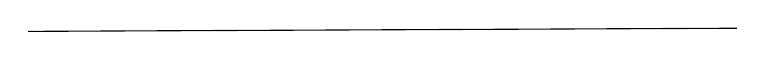
\begin{tikzpicture}\draw (0,0)--(9,0.04);\end{tikzpicture}}

\figure{
\begin{tikzpicture}[baseline=(n.base)]
\node (n) at (0,0) {$8^{\circ}$};
\draw (0,0) ellipse (0.35 and 0.31);
\end{tikzpicture}}
Si $U$ est un élément de $\mathcal{M}_{\rho,\sigma}$, on lui
associe ses images par $\Theta=\Theta_G$, $\Theta_\rho$, $\Theta_\sigma$, et par
\deleted{$\unsure{\varepsilon_3,\varepsilon_2}$}
$\chi$, $\varepsilon_3$, $\varepsilon_2$, on les note respectivement
\[
\tag{152}
\left\{\begin{array}{l}
\uline{U}\in\Gamma G\\[4pt]
\uline{a}\ \unsure{\in}\Gamma T_\rho\\[4pt]
\uline{b}\in\Gamma N'_\sigma\\[4pt]
\figure{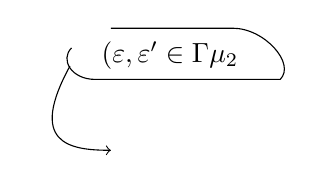
\begin{tikzpicture}[baseline=(e.base)]
\node[inner sep=3pt] (e) at (0,0) {$(\varepsilon,\varepsilon'\in\Gamma\mu_2$};
\draw (-1.25,0.1) .. controls (-1.4,-0.05) and (-1.25,-0.3) .. (-0.95,-0.3)
 -- (1.4,-0.3) .. controls (1.6,-0.1) and (1.2,0.35) .. (0.8,0.35) -- (-0.75,0.35);
\draw[->] (-1.27,-0.13) .. controls (-1.8,-1.1) and (-1.3,-1.2) .. (-0.75,-1.2);
\end{tikzpicture}}\\[4pt]
\mu\in\Gamma G_m
\end{array}\right.
\]

\margin{\unsure{satisfaisant}
\[
\tag{152'}
\left\{\begin{aligned}
\mu&=\delta_G(\uline{U})=\unsure{\delta'_\sigma|\delta_\sigma}(\uline{b})=\varepsilon'\delta_\rho(a)\\
\varepsilon&=\varepsilon_\sigma(\uline{b})
\end{aligned}\right.
\]
donc ces quantités sont déterminées par la seule
\unsure{conn.} de $\uline{U},\uline{a},\uline{b}$}

\margin{\figure{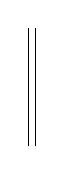
\begin{tikzpicture}
\draw (0,0)--(0,1.5);\draw (0.09,0)--(0.09,1.5);
\end{tikzpicture}}
Il faudrait expliciter que les \unsure{égalités|relations} (152)' \uline{caractérisent}
$\mathcal{M}_{\rho,\sigma}$ comme sous-groupe de $G\times T_\rho\times N'_\sigma$
-- il faudrait faire la vérification, pour se rendre
compte \unsure{si on n'a pas} \unsure{oublié}, dans
\unsure{(135)} des \unsure{hyp$^{\mathrm{ses}}$} à faire\ldots}

\margin{\uline{NB} $G^{\pm1}\overset{\mathrm{d\acute ef}}{=}\operatorname{Ker}\delta_G^2$}

avec des notations du \S\ 46 et suivants.
\unsure{manquent} cependant, dans l'optique \unsure{des} \unsure{points entiers},
les éléments notés précédemment
\diagram{\begin{tikzcd}[ampersand replacement=\&,column sep=small,row sep=small]
\uline{u} \& \alpha \& \beta \& \alpha_0 \& \beta_0 \& f\arrow[lllll,bend right=28]
\end{tikzcd}}
, avec
\[
\left|\begin{aligned}
u&\in\Gamma\unsure{T_0}\subset\Gamma G\\
\alpha,\alpha_0&\in\Gamma G^{\pm1}\subset\Gamma G\\
\beta,\beta_0,f&\in\Gamma SG.
\end{aligned}\right.
\]
reliés \inserted{entre eux et aux précédents,} par des relations
\[
\left\{\diagram{\begin{tikzcd}[ampersand replacement=\&,row sep=small,column sep=normal]
\alpha=\uline{u}\,\uline{a}^{-1}
\& {}\arrow[d,dash,start anchor=north,end anchor=south]
\& |[yshift=-0.8em]|{\text{i.e.}\quad\uline{u}=\alpha\unsure{\overline{a}}=\beta b.}\\
\beta=\uline{u}\,\uline{b}^{-1} \& {} \& \\
\uline{U}=f^{-1}\uline{u}
\arrow[uu,bend left=80,start anchor=west,end anchor=west]
\arrow[u,bend left=70,start anchor=west,end anchor=west] \& \& \\
\alpha_0=f^{-1}\alpha \& \& \text{i.e.}\quad\alpha=f\alpha_0\\
\beta_0=f^{-1}\beta \& \& \text{i.e.}\quad\beta=f\beta_0
\end{tikzcd}}\right.
\]
\margin{formules \uline{dans $G$}}

\margin{\uline{NB} de ces \unsure{6 quantités} (153),
$\uline{u}$ est distingué par le fait d'être
\uline{\unsure{multiplicatif}}
(comme les quantités (152))}

\margin{On pourrait introduire
\[
\left\{\begin{aligned}
\xi&=\alpha\rho(\alpha)^{-1}\\
\eta&=\unsure{\varepsilon}\,\beta\sigma(\beta)^{-1}
\end{aligned}\right.
\quad\unsure{(153)}
\]
\[
\begin{aligned}
g&=\alpha_0\rho(\alpha_0)^{-1}\\
h&=\unsure{\varepsilon}\,\beta_0\unsure{\sigma}(\beta_0)^{-1}
\end{aligned}
\]
mais \unsure{peu} nous \unsure{chaut} ici.}

\mspage{452}

\begin{center}
{\small
452\\
\texttt{https://grothendieck.umontpellier.fr}\\
Université de Montpellier, UMR CNRS 5149, Case courrier 051, Place Eugène Bataillon\\
34095 Montpellier cedex 5 - France
}
\end{center}
